Quantum key distribution (QKD) is a technique that allows two parties to share a
common secret key that can be used for encryption, on Alice’s part, and decryption,
on Bob's, so that, while being transmitted, the data remains incomprehensible to any observer 
who does not know the key.
\begin{figure}[!h]
\centering
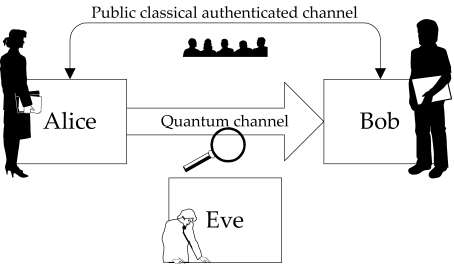
\includegraphics[width=\textwidth,height=\textheight,keepaspectratio]{3.png}
\caption{QKD overview}
\label{fig3}
\end{figure}
As mentioned earlier, the main idea of how key-confidentiality is ensured revolves around the quantum mechanical principles
wherein if Eve tries to determine the key, it is sure that she will be detected by the parties 
(who will then go on to discard the key). If however, no tapping attempt is made, the secrecy of the distributed key 
is guaranteed.

QKD requires a non-classical transmission channel on which quantum particles can be transmitted between Alice and Bob. 
Although, theoretically, any quantum particle can be used, in practice, those carriers are usually photons, with the
channel being either an optical fiber or the open air.
In the photons, Alice will encode random bits of information that will make up the key, so that no Eve can 
predict any of the transmitted key-bits.
For simplicity's sake, it will be presupposed that ``truly random" bits ($0$s and $1$s) are used.
After the transmission, Alice and Bob will compare bases and will only keep the identical-basis bits (a process called {\it sifting}), 
a fraction of which will then be checked for transmission errors (a process called {\it error correction}),
including ones caused by eavesdropping.
In such a case, no fundamental problem arises, as any Eve is guaranteeably detectable 
(through {\it error correction}), after which Alice and Bob, only in the worst case scenario, will need to recover a fresh secret key, 
out of the bits that are unknown to Eve or regenerate one anew, choices depending on pre-decided bit-error threshold parameters.
To make things easier, it is assumed, that Alice and Bob do not have access to a
private channel (as is the case in most realistic scenarios where applicability is to be
sought after), with a public classical authenticated channel being used, instead.
It has been proven that the confidentiality of data is absolutely guaranteed when
the length of the encryption key is as long as the message to be transmitted and it is never
reused for future messages; that is where the usefulness of QKD comes into effect.

To be more precise, the confidentiality of the transmitted data is ensured by two parts: the
quantum-distributed key and the encryption protocol. QKD is only
responsible for key distribution, meaning that its goal is guaranteeing the secrecy of a
distributed key. Extra mechanisms involving the manipulation of the data
(encryption/decryption - with the help of that secret key), will be discussed with the BB84
and E91 protocols, to be glimpsed upon further on.
